\documentclass[DIV10]{scrartcl}

\usepackage[utf8]{inputenc}
\usepackage{url}
\usepackage{hyperref}
\usepackage{graphicx}
\usepackage{enumerate}
  
\makeatletter
\newcommand*{\tol}[1]{$\overline{\hbox{#1}}\m@th$}
\makeatother

\renewcommand{\arraystretch}{1.2}

\author{jmA500 <jm@metweb.de>}
\date{\today}
\title{Keyboard tap to configure an Amiga 500}

\begin{document}
\maketitle
\section{Description}
This little piece of hardware is used to provide some means for
configuring an Amiga 500 with the keyboard. This is to replace at
least some of the small switches that are commonly used to configure
the extensions in an Amiga. The circuit listens to the keys pressed
on the Amiga keyboard and then adjusts some of its output pins. These
pins connect to jumper headers on the extension boards and hence provide some
means to configure these extensions without opening the case or
drilling holes into it.
\begin{center}
  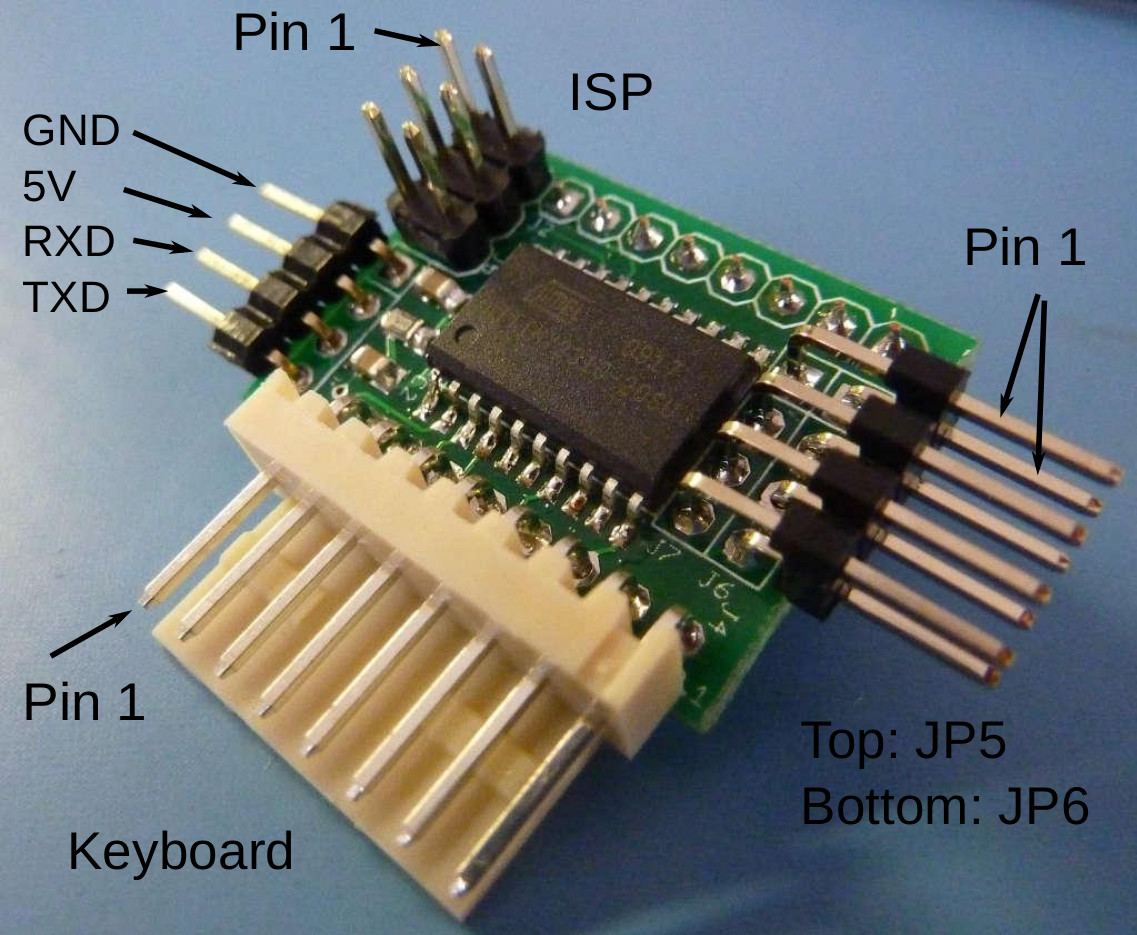
\includegraphics[width=.7\linewidth]{config-annot}
\end{center}
Note however, that this project is not for beginners. If you have
other extensions than I have, you will likely have to adapt the
firmware to your needs. Also, you have to figure out whether your
extensions are configurable by means of an external MCU, that is if is
suffices to drive a signal statically high or low. Switching a dynamic
signal is not possible (without extra hardware)\footnote{I have seen
  some kickstart switches that use a switch to route a signal to
  either of the two ROMs.} 

In any case you need a possibility to program the AtTiny2313
micro-controller with an in system programmer (ISP). These are cheaply
available and connect to USB or parallel port. A lot of information
regarding this micro-controller can be obtained on the
excellent websites \url{http://www.avrfreaks.net/} or
\url{http://www.mikrocontroller.net/} (German).

In addition, if you are not running a Linux machine similar to mine
there might be some extra difficulties adapting the code to your build
environment. In particular I am not using AVR studio and this
distribution does not include any project file for it. However,
pre-built firmware images are included, if you are happy with the
firmware out of the box.

\section{Disclaimer}
I am not responsible for any damages done by this device, and I do not
guarantee that it will work at all. Only connect this to your precious
Amiga, if you are sure about what it does, how it works, and whether
the firmware is what I claim it to be.

\section{Acknowledgments}
The idea to this project was born during a discussion in the
\url{a1k.org/forum} and was suggested by Paradroid. However, if I did
not have all the great hardware extensions created by the community
I would not have had any reason to start the project. Thanks also to
the members of the a1k.org forum encouraging me to continue this project.

\section{License}
All parts of this project are free to use in non-commercial
projects. The firmware is licensed under terms of the GPL 2. Please
quote this document in any derived work. See the file COPYRIGHT in
\verb#src/attiny4313# for additional information, in particular the
reference to Peter Fleury who provided a neat UART library for the
Atmel MCUs.

\section{Hardware}
The hardware is plain and simple, an AtTiny4313 (or 2313) in
minimal configuration with a few pin headers to connect the
configuration jumpers and an ISP Programmer.
In addition, the RxD and TxD pins are accessible on additional
pins.
\begin{center}
  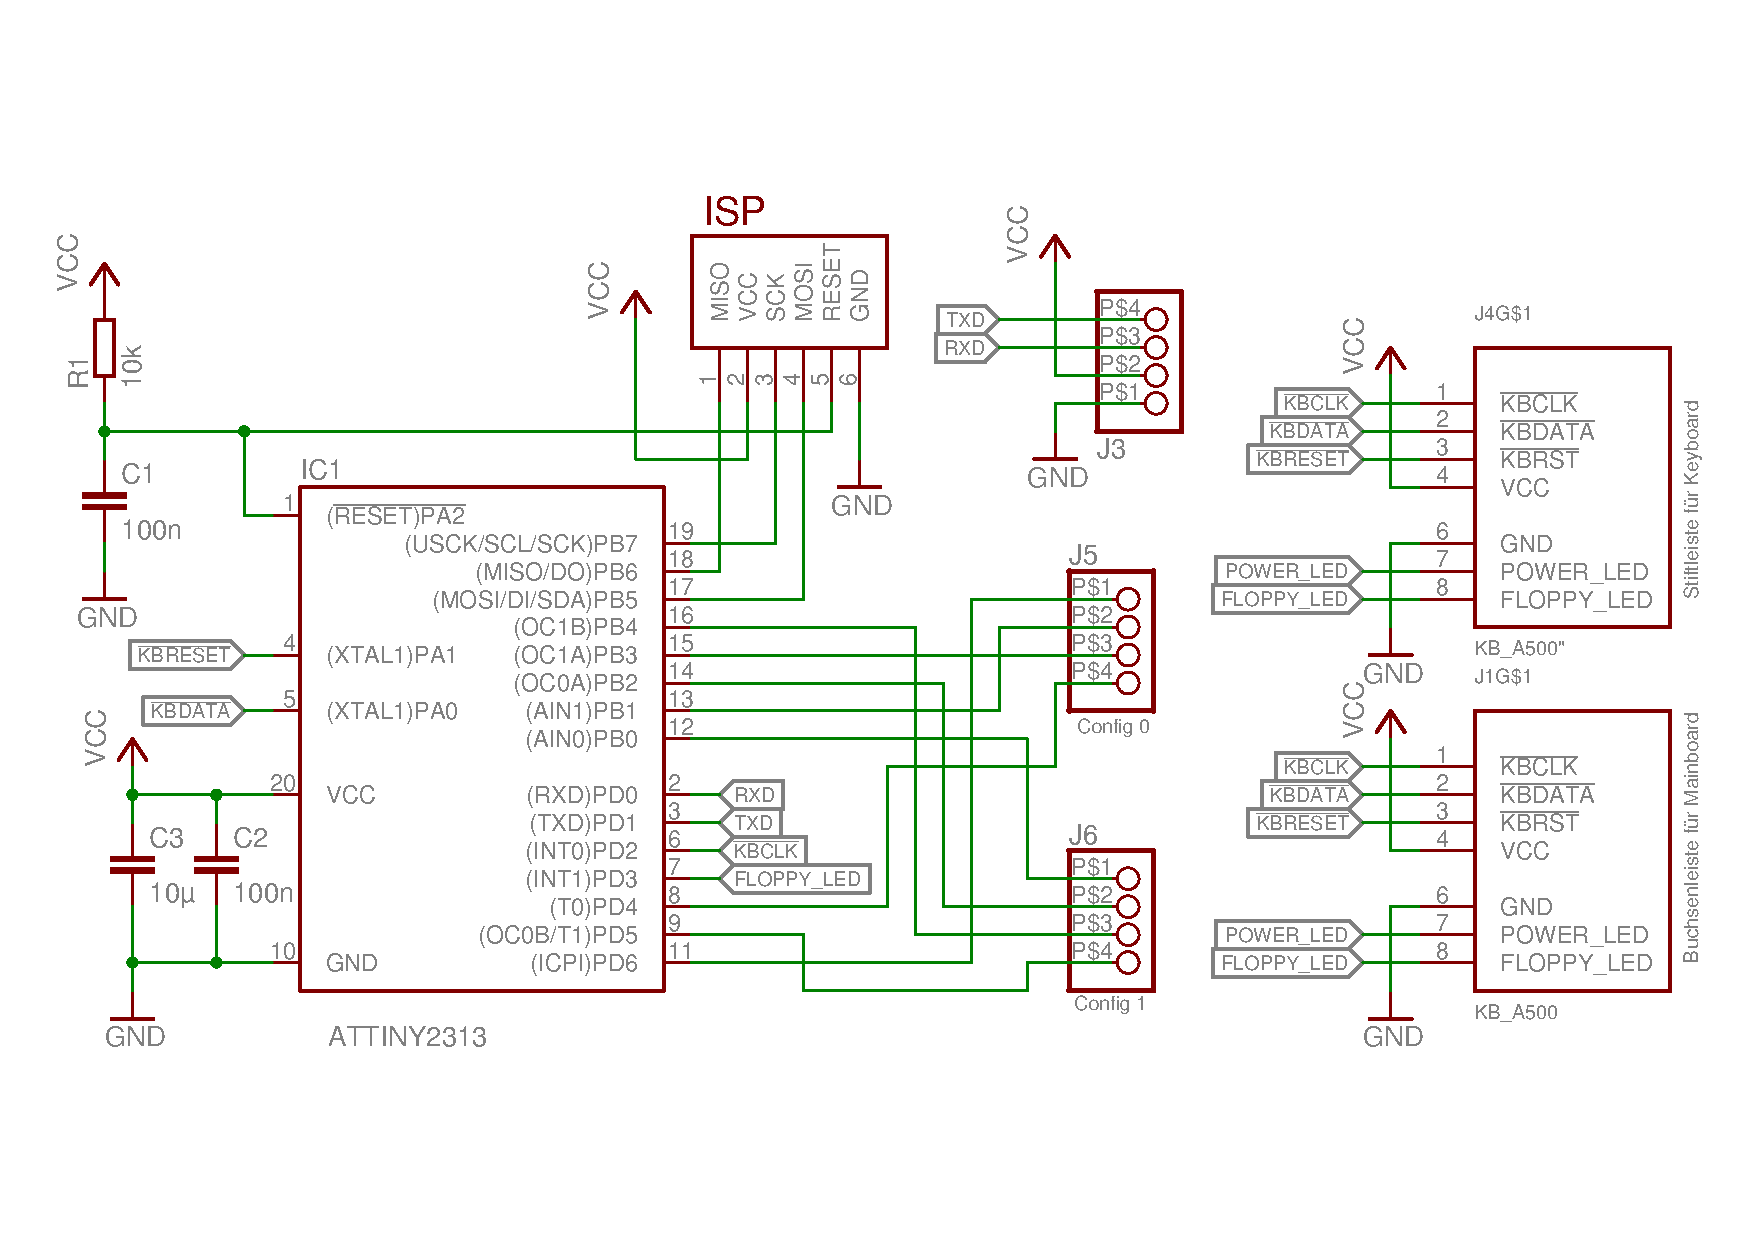
\includegraphics[width=.7\linewidth]{../hardware/schematic.pdf}
\end{center}
There is a board layout done in such a way that the little PCB can be
directly fitted on the keyboard connector on the mainboard of an Amiga
500(+).

However, the whole circuit is so simple that you might consider
building it without a PCB, or you might use an Ardiuno or something
similar. 

\subsection{Part list}
\begin{center}
  \begin{tabular}{|l|l|l|}
    \hline
    IC1 & AtTiny 2313 SO or AtTiny 4313 SO\\
    \hline
    C1,C2 & 100n SMD 0805 \\
    C3 & 10$\mu$ SMD 1206 \\
    R1 & 10k SMD 0805 \\
    \hline
    J1  & 1x8 socket strip 180$^\circ$ 2.54\\
    J2  & 2x3 pinheader 180$^\circ$ 2.54\\
    J3  & 1x4 pinheader 180$^\circ$ 2.54\\
    J4  & 1x8 pinheader 90$^\circ$ 2.54\\
    J5,J6  & 2x4 pinheader 90$^\circ$ 2.54\\
    \hline
  \end{tabular}
\end{center}
For future extensions I suggest using a 4313 with 4k flash and 256
bytes of RAM if you can get one. The current firmware barely fits the
2313 as it uses about 1984 bytes of its 2k flash memory. On the other
hand, approximately half of this is for the UART input/output
functions that you may or may not find useful. Note that I did not
test the board with a 2313{\bfseries A} although that might work
without changing the code.

\subsection{Pin Configuration}
\subsubsection{J1: Connects to A500 mainboard}
\begin{center}
  \begin{tabular}{|l|l|}
  \hline
    1 & \tol{KBCLK} \\
    2 & \tol{KBDATA} \\
    3 & \tol{KBRESET} \\
    4 & VCC \\
    5 & \\
    6 & GND \\
    7 & POWER\_LED \\
    8 & FLOPPY\_LED \\
    \hline
  \end{tabular}
\end{center}
\subsubsection{J2: ISP}
This is to connect an ISP programmer. The pin-out corresponds to Atmel 6-pin
ISP connector. {\bfseries Please make sure that the programmer does not power the
MCU when connected to the A500 mainboard.}
\begin{center}
  \begin{tabular}{|l|l|}
    \hline
    1 & MISO\\
    2 & VCC\\
    3 & SCK\\
    4 & MOSI\\
    5 & \tol{RESET}\\
    6 & GND\\ \hline
  \end{tabular}
\end{center}

\subsubsection{J3: Serial connector}
This is a serial connection with 5V logic levels. Names are from the
perspective of the MCU, so you have to connect the TxD of your
computer to the RxD on the PCB.
\begin{center}
  \begin{tabular}{|l|l|}
    \hline
    1 & GND \\
    2 & VCC \\
    3 & RxD \\
    4 & TxD \\ \hline
  \end{tabular}
\end{center}
The firmware will output some status messages here, and listens to
commands via a small parser. Have a look at the software how to use
it (or send the string \verb#help# to see a small help message). 

\subsubsection{J4:  Connect your keyboard here}
Same as J1.

\subsection{J5, J6: Connectors for configuration jumpers}
\label{sec:config-jumpers}
These connectors provide 8 pins to configure the hardware. Everything
that happens on these pins depends on the firmware. The software
provided with this documentation emulates open collector outputs, ie.\
it will either pull pins low or let them float (configure as inputs)
but never pull them high.

My Amiga 500 is equipped with a configurable 1.8/2MB Ranger memory
extension \cite{Memory}, a Kickflash \cite{Kickflash-Thread,Kickflash-Manual} and
the 68010@14MHz Turbo card by Matze \cite{Turbokarte}. The 
configurator is used to configure all three extensions. The memory
extension is connected to J5, Kickflash and Turbo card to J6 as
follows:
\begin{center}
  \begin{tabular}{|ll|l|}
    \hline
    J5 & 1 & EXRAM \\
    & 2 & CHIPRAM \\
    & 3 & CONF0 \\
    & 4 & CONF1 \\
    \hline
    J6 & 1 & Kickflash (DIP Switch 3) \\
    & 2 & Kickflash (DIP Switch 4) \\
    & 3 & Turbo Card \\
    & 4 &
    \\ \hline
  \end{tabular}
\end{center}
\begin{enumerate}[Note 1:]
\item \label{item:remark-memory} If you do not own one of the memory expansion boards that I am
  talking about, you can connect JP5-1 to the on/off switch of a 512k
  memory expansion card and use F1/F2/F3 to turn it on and F4/F5 to
  turn it off.
\item The Kickflash has a MCU on it which must be disabled by removing
  it or cutting its power.
\item My version of Matze's Turbo card needs one extra pull-up
  resistor on the configuration pin to be configurable with the emulated
  open collector outputs.
\end{enumerate}

\section{Firmware}
The firmware for the Atmel is written in C and compiles with avr-gcc
4.8.2 but may or may not compile with different versions although I
tried to be as compatible as possible. The directory \verb#firmware#
contains precompiled flash and eeprom images in Hex-format for the
AtTiny 2313 and 4313. For both MCUs the fuses setting is
\begin{quote}
  \verb#LFUSE = 0xD4, HFUSE = 0xDB, EFUSE = 0xFF#.
\end{quote}
Make sure to program both the flash memory with the corresponding
\verb#.hex# file and the eeprom memory with the \verb#.eep#
file. Never attempt to flash the MCU while plugged into a running
Amiga 500, since it will switch configuration when finished
programming. This could damage your Amiga.


The Makefile provided in the \texttt{src} directory should do the job
by simply running \texttt{make}. If compiling for an AtTiny2313 you
must adjust the \texttt{MCU} variable in the Makefile to read
\texttt{MCU = attiny2313}. If you happen to have a USBasp ISP
programmer \cite{USBasp} you can program the MCU by simply running
\texttt{make fuses} and \texttt{make program}. The Makefile supports
programming with avrdude, the programmer is selected with the variable
\verb#AVRDUDE_PROG#. 

The source code should be mostly self explanatory\footnote{An
  obviously biased judgment YMMV.}, although small code
has been preferred to readable code in some places. The crucial global
variable is \verb#conf_data# an array of bytes. This contains the
mapping of F-keys to actual configuration. Since I use the software to
configure three extensions, also the bytes in this array are split
into three parts. The lower four bits correspond to the configurations
of the memory extension using 4 jumpers. The first entry in
\verb#conf_data# is selected via F1, the second by F2, and so on, up
to F10. The index of the current configuration is stored in the global
variable \verb#conf.current[0]#, the next selection in
\verb#conf.next[0]#.  The lower four bits of \verb#conf_data# the are
then used to set the pins of J5. {\bfseries A one in these bits
  results in pulling the corresponding pin low.}

The second extension to configure is the Kickflash. It uses two
jumpers and is connected to J6-1 and J6-2. The index of the next
configuration is in \verb#conf.next[1]# and selectable by Shift-F1
to Shift-F4. The settings for these jumpers are stored in bits 4 and 5
of \verb#conf_data[conf.next[0]]#. See the function
\verb#set_config()# in \verb#main.c# for details.

Bit 6 of the \verb#conf_data# entries is used to enable or disable the
turbo card. This bit corresponds to Shift-F6 and Shift-F7. Selecting
the configuration with Shift-F6 results in setting \verb#conf.next[2]#
to \verb#0#. Since bit 6 in \verb#conf_data[0]# is set, J6-3 will be
pulled low on the next reset and hence the turbo card is
disabled. Selecting the next configuration with Shift-F7 results in
\verb#conf.next[2]# being \verb#1#, and since bit 6 in
\verb#conf_data[1]# is not set, J6-3 will be left floating on the next
reset and hence the turbo card is enabled.

\section{Usage}
This is the selections available if the configurator is connected as
described in section~\ref{sec:config-jumpers} and with the default
firmware. The keys F1-F10 are used to configure the memory expansion:
\begin{center}
  \begin{tabular}{|l|l|}
    \hline
    F1 & Select + 512kB Chipram and + 1.5MB Slow RAM \\
    F2 & Select + 512kB Chipram and + 1 MB Slow RAM \\
    F3 & Select + 512kB Chipram and + 0.5MB Slow RAM \\
    F4 & Select + 512kB Chipram and + 0 MB Slow RAM \\
    F5 & Select + 0kB Chipram and + 0 MB Slow RAM \\
    F6 & Select + 0kB Chipram and + 1.8 MB Slow RAM \\
    F7 & Select + 0kB Chipram and + 1.5 MB Slow RAM \\
    F8 & Select + 0kB Chipram and + 1.0 MB Slow RAM \\
    F9 & Select + 0kB Chipram and + 0.5 MB Slow RAM \\
    F10 & Select + 0kB Chipram and + 0 MB Slow RAM \\
    \hline
  \end{tabular}
\end{center}
If you do not have this memory expansion board,
cf.~\ref{item:remark-memory} in section~\ref{sec:config-jumpers}.

With keys Shift-F1 to Shift-F4 the Kickflash is configured:
\begin{center}
  \begin{tabular}{|l|l|}
    \hline
    Shift-F1 & Kickflash Slot 0\\
    Shift-F2 & Kickflash Slot 1\\
    Shift-F3 & Kickflash Slot 2\\
    Shift-F4 & Kickflash Slot 3\\
    \hline
  \end{tabular}
\end{center}
Keys Shift-F6 and Shift-F7 configure the turbo card (actually its CPU
frequency):
\begin{center}
  \begin{tabular}{|l|l|}
    \hline
    Shift-F6 & Turbo Mode off (7.x MHz)\\
    Shift-F7 & Turbo Mode on (14.x MHz) \\
    \hline
  \end{tabular}
\end{center}
To select a configuration push the key combination desired and
afterwards the Help-Key three times in a row. The configuration is not
executed immediately but only after a keyboard reset. Thus one can
configure all three extensions to a different state before
reset. However, each of the three configurations requires to press
three times Help. Note that not all configurations are valid, for
example Kickstart 1.2 will not run with 1.5 MB of Slow RAM. My
Kickflash has Kickstart 1.2 in slot 2 (corresponding to
Shift-F3). When switching configurations the firmware checks whether the
memory configuration is incompatible (F1 or F7) and if so, switches
the kickstart to slot 0. This might be considered a bug, but actually
is a feature.

Moreover, the 1.8 MB setting is incompatible with some IDE interfaces
due to address conflicts. Also some configurations will not start
immediately or will not be recognized after a simple keyboard (warm)
reset. Any Kickstart below and including 1.3 will show a yellow screen
if the amount of available memory is decreased, and increased memory
is not recognized. Thus a power cycle is needed.

If you accidentally select a configuration that does not run and is
screwed in such a way that the keyboard is not initialized, you can do
a keyboard reset for at least 6 seconds to load the hopefully save
configuration (F1, Shift-F1, Shift-F6).

\bibliographystyle{plain}
\bibliography{references}

\end{document}

%%% Local Variables: 
%%% mode: latex
%%% TeX-master: t
%%% End: 
